\documentclass[graphics]{beamer}

\usepackage{graphicx}
\usepackage{verbatim}
\usepackage{wrapfig}
\useoutertheme{shadow}
%\usecolortheme{orchid}
\usecolortheme{seahorse}
\usepackage{tikzsymbols}
\usepackage{textcomp}
\usepackage{parskip}

% math commands
\newcommand{\be}{\begin{eqnarray}}
\newcommand{\ee}{\end{eqnarray}}
\newcommand{\beq}{\begin{equation}}
\newcommand{\eeq}{\end{equation}}
\def\simless{\mathbin{\lower 3pt\hbox
      {$\rlap{\raise 5pt\hbox{$\char'074$}}\mathchar"7218$}}}
\def\simgreat{\mathbin{\lower 3pt\hbox
      {$\rlap{\raise 5pt\hbox{$\char'076$}}\mathchar"7218$}}} %> or of order

% variables

\def\toonscale{0.45}
\def\mboxy#1{\mbox{\small #1}}


\begin{comment}
\AtBeginSection[]{
  \frame{
    \frametitle{Outline}
    \tableofcontents[currentsection]
  }
}
\end{comment}

\title{Cosmic the origin of angular momentum verified through galaxy
  zoo: frozen fossils of the initial conditions
}
\subtitle{}
\author[U. Pen]{\textcolor{green}{Ue-Li Pen, ASIAA, CITA}
\\[8mm] 
}
\date{March 10, 2023}


\begin{document}

\frame{
\begin{picture}(320,250)
\put(-50,-130){
\includegraphics[width=5.5in]{Figures/delta_nu_sim.pdf}}
\end{picture}
\vspace{-3in}
\titlepage
}

%\section*{Introduction}
\section{The origin of angular momentum
}

\begin{comment}
  \subsection{Outline}

  \frame{
    \frametitle{Outline}
    \tableofcontents
  }
\end{comment}

   \frame{
    \frametitle{Galaxy Spins}
    \begin{itemize}
        \item most galaxies are rotating disks of stars and gas
        \item dust lanes, trailing spiral arms, HI velocity (rotation) field
        \item readily identifyable spin axis in 3-D: observable vector field 
        \item spin direction well preserved from initial conditions, $\sim$ 0.5 correlation with primordial IC.   {\it conservation of angular momentum}
        \item potentially vast reservoir of fossils from initial conditions ($\gtrsim 10^8$ modes)
        \item direct probe of primordial helicity, cosmic neutrino background
     \end{itemize}
}
\frame{
    \frametitle{Observable}
\includegraphics[width=4.1in]{Figures/M51s.jpg}  

(M51, from Wikipedia)
  }
\frame{
    \frametitle{Torquing}
\vspace{-0.1in}
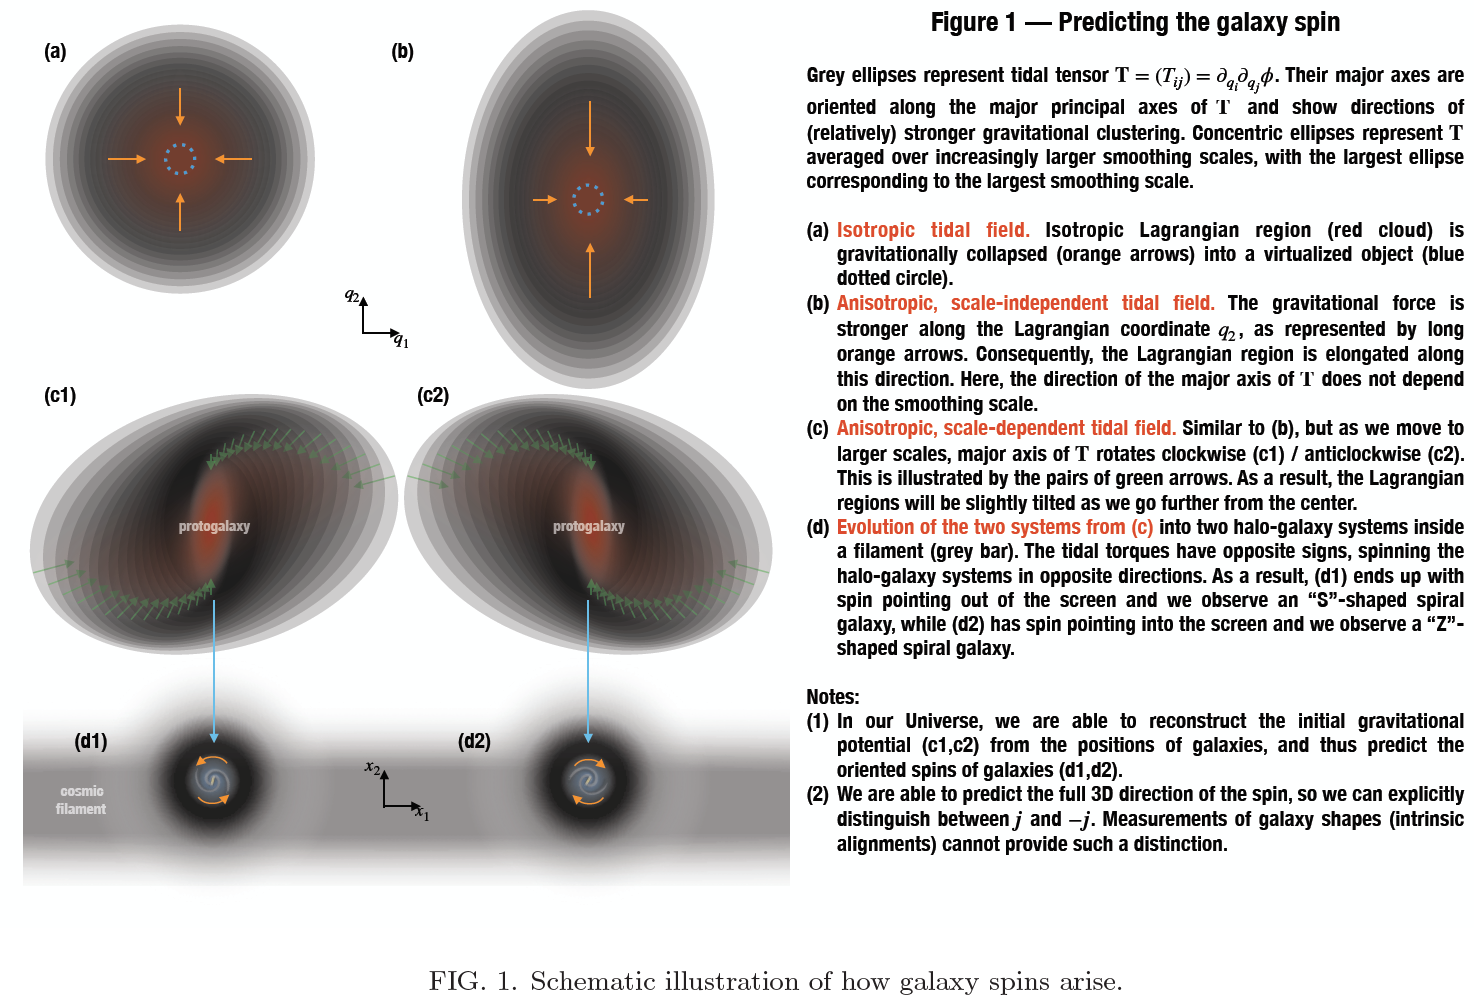
\includegraphics[width=4.5in]{Figures/torque.png}

Motloch+ 2003.04800
  }


\frame{
    \frametitle{Projection}
\vspace{-0.1in}\hspace{-0.6in}
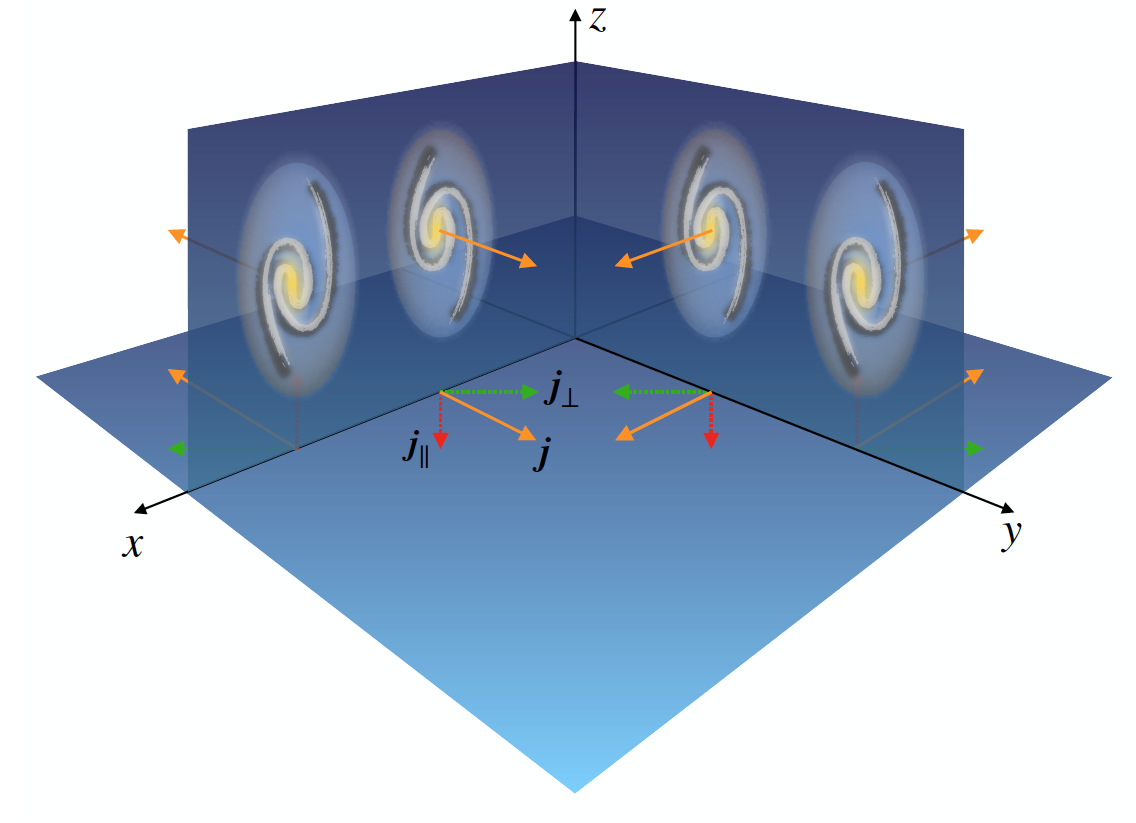
\includegraphics[width=2.9in]{Figures/fourfold.png}
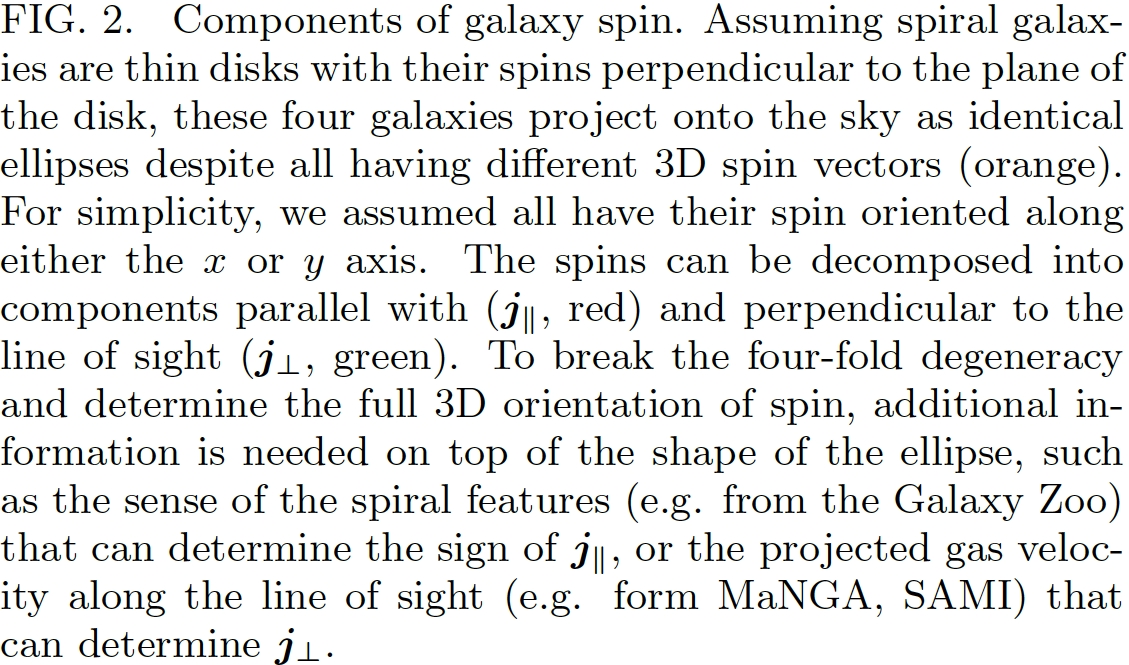
\includegraphics[width=1.9in]{Figures/fourfoldcaption.png}

  }


\frame{
    \frametitle{Prograde Winding}
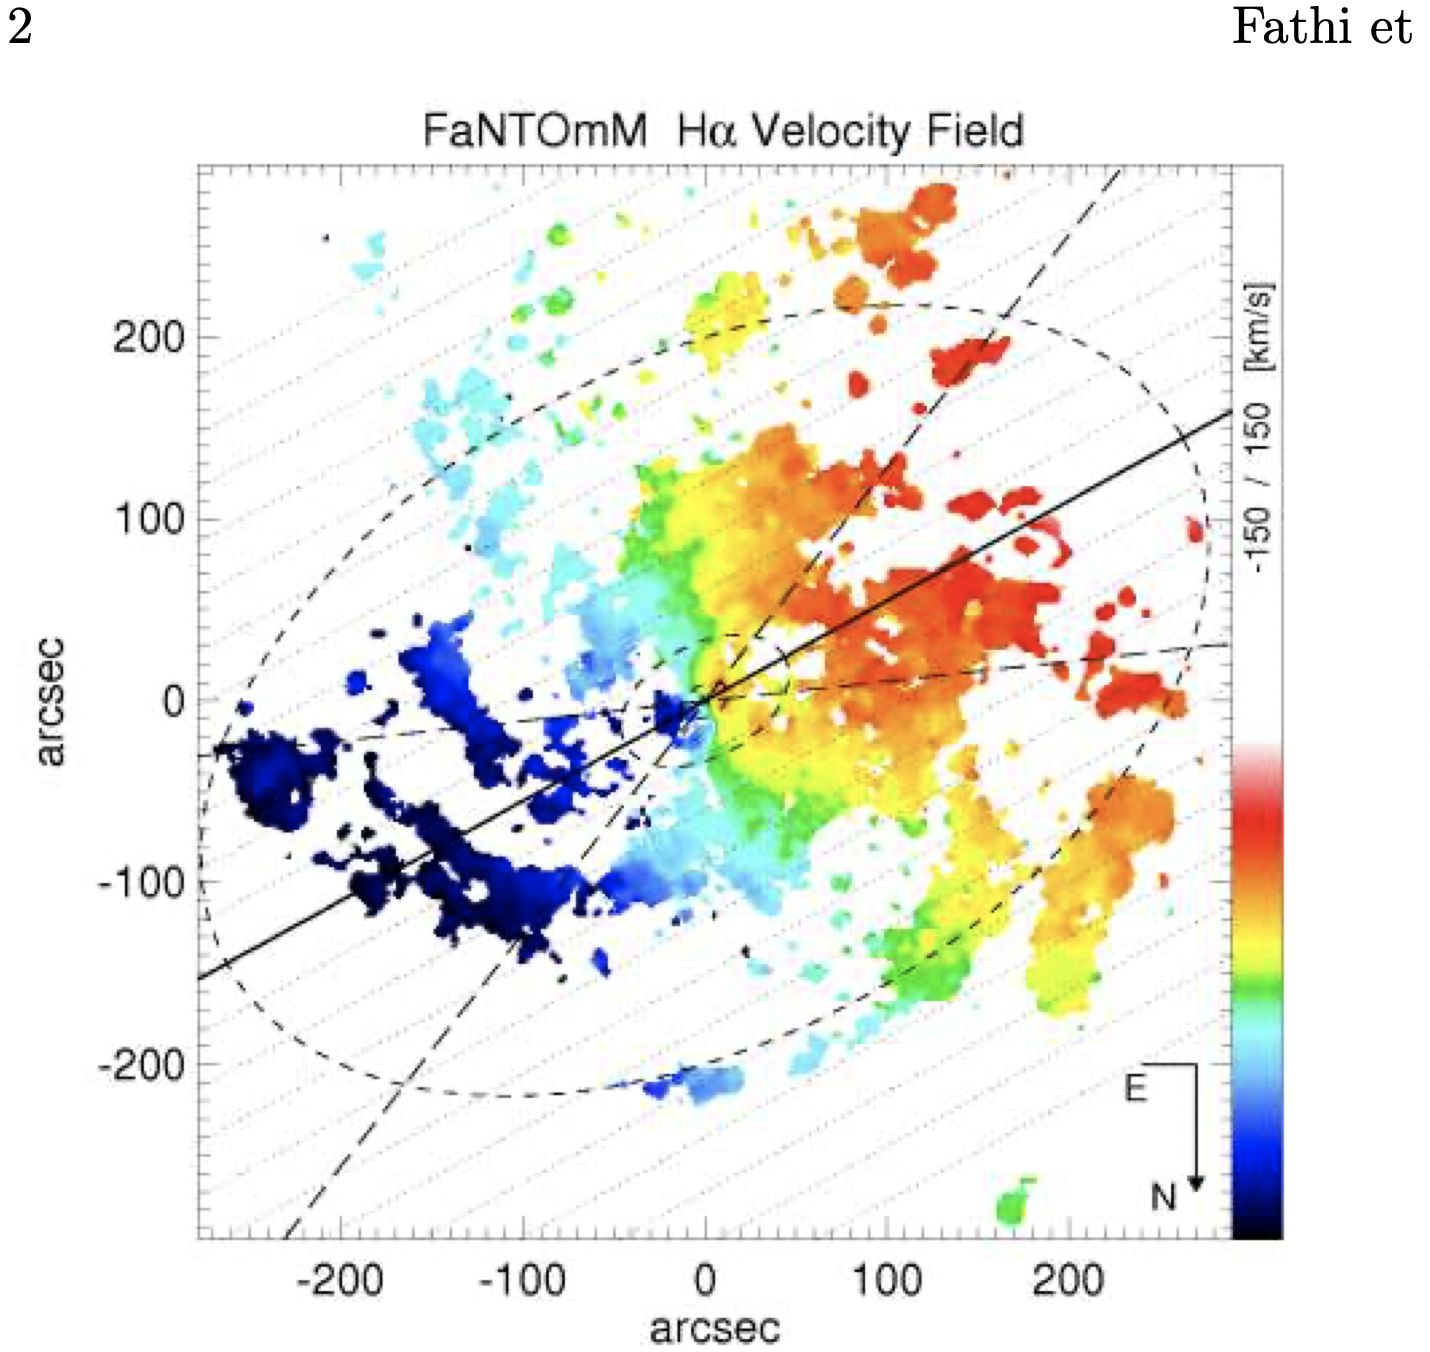
\includegraphics[width=3.1in]{Figures/fantomm.png}  

(NGC6946, from Fathi+ 2007)
  }
%\frame{
 %   \frametitle{Tilt}
%\includegraphics[width=4.1in]{Figures/SAMI.png}  
%(SAMI, 1409.4147)
 % }

  \frame{
    \frametitle{Observables}
    \begin{itemize}
        \item ellipticity
        \item position angle
        \item winding direction (S vs Z)
        \item reddening
        \item human and machine classifications for $10^{4-6}$ objects
          (galaxy zoo, Land+ 2008 )
    \end{itemize}
}


\frame{
    \frametitle{Zoo}
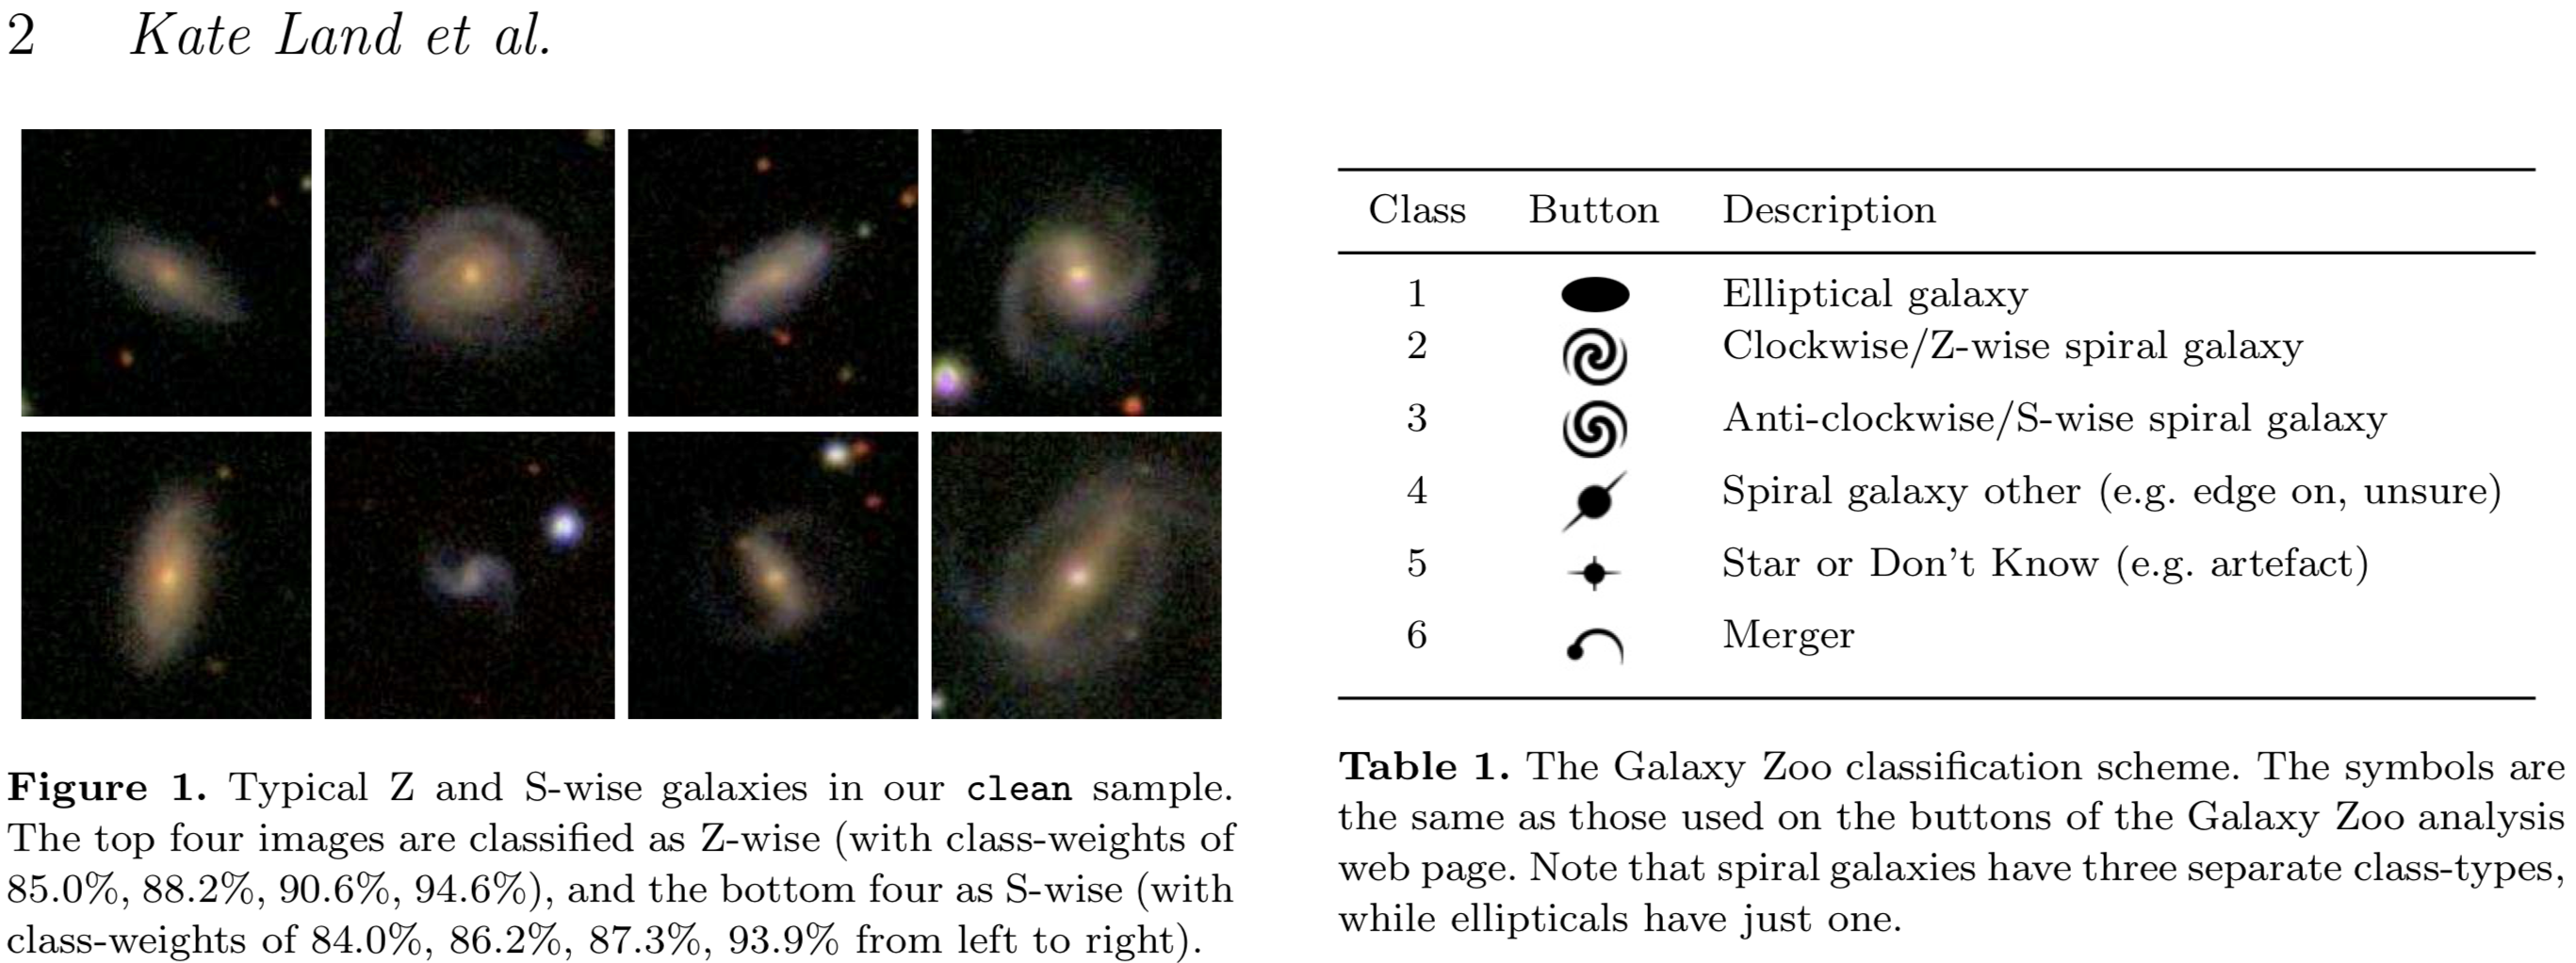
\includegraphics[width=4.1in]{Figures/land2008.png}  
  }

  \frame{
    \frametitle{Angular momentum (``spin'')}
    \begin{itemize}
        \item 1st order effect from misalignment of moment of inertia
          and tidal tensor
        \item torque: $\tau\equiv\int \rho \bf{r} \times \nabla \phi$
        \item Taylor expand: $\tau_i=\epsilon_{ijk} \int \rho x^jx^l \partial_l\partial_k\phi \equiv\epsilon_{ijk} I_{il}T_{lk}$
        \item Tensor form $\tau= * I \cdot T$
        \item first realized by S. White (1984), see also LP00
     \end{itemize}
}
 
\frame{
    \frametitle{3-D: E-mode Lagrangian}
%\vspace{-0.5in}
\hspace{-0.2in}\includegraphics[width=2.1in]{Figures/nonlinear.png}  
\vspace{0.15in}\includegraphics[width=2.1in]{Figures/reconstructed.png}  

Eulerian (L) vs Lagrangian (R) (from Yu et al 2016, 1610.7112)
  }

 \frame{
    \frametitle{Predicting Neutrino Torques}
    \begin{itemize}
      \item $\nu$ gravitational field (large scale tide) torques CDM (small scale inertia)
      \item $\Delta x (q) = q^j \partial_i\partial_j \psi$
        \item $I_c \sim T_c$: both describe particle displacement
        \item $j_\nu = \epsilon I_c T_\nu \sim  \epsilon T_c T_\nu$
        \item Neutrino tidal torque is predictable observable from
          displacement potential
     \end{itemize}
 }
 
  \frame{
    \frametitle{Illustration}
\vspace{-0.5in}\hspace{-0.6in}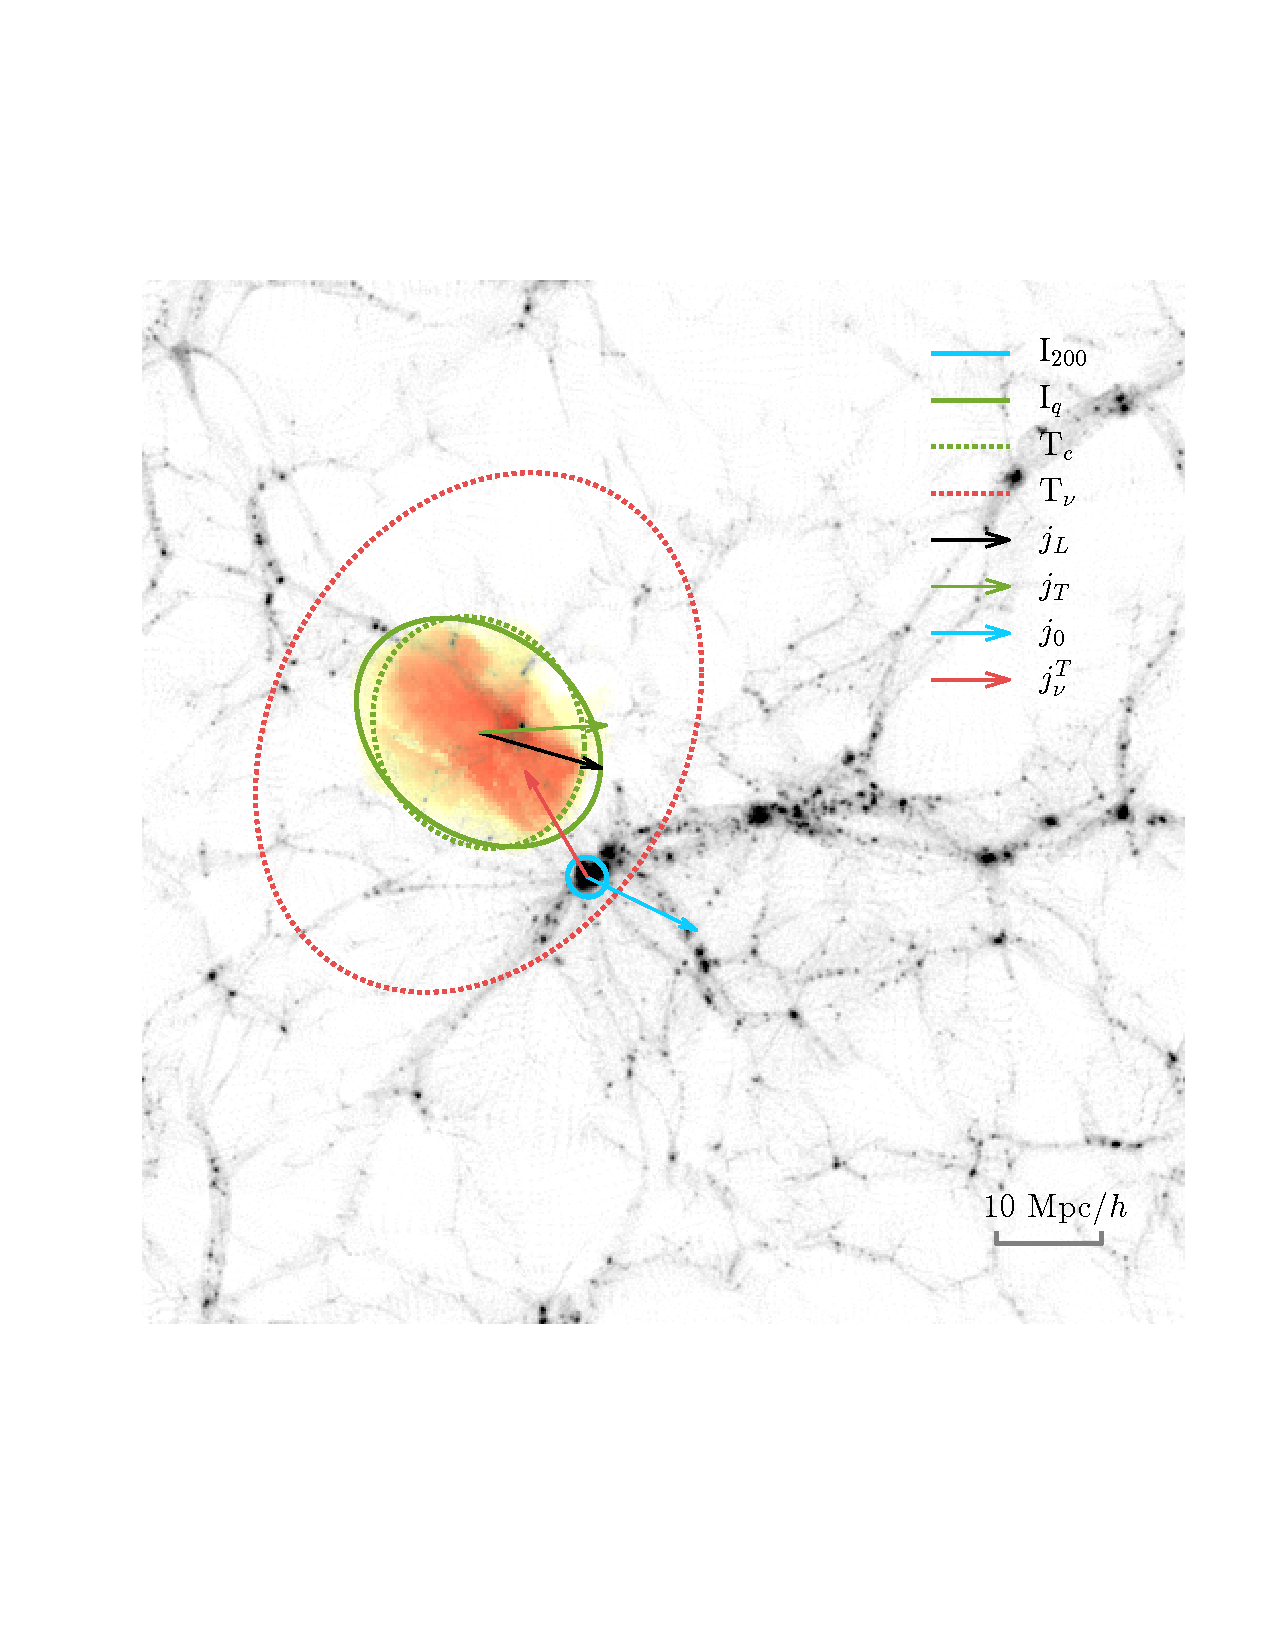
\includegraphics[width=5.0in]{Figures/f1.pdf}
}

 \frame{
    \frametitle{Size estimate}
    \begin{itemize}
    \item $|j_\nu/j_c| \sim 10^{-4} (f_\nu /0.003) [\sqrt{P(k_{\rm FS})/P(k_{\rm vir})}/0.03]$
    \item agrees with simulation measurement
    \item need $n> 10^8$ galaxy spins
    \item accessible in next generation 21cm surveys
     \end{itemize}
  }

  \frame{
%\vspace{-0.5in}
    \frametitle{predicting CDM spin}
    \begin{itemize}
    \item Tidal Torque Theory (TTT): relates spin to initial Inertia and Tide
    \item Inertia tensor not easily identified, requires running N-body simulation.
    \item approximate Inertia by Tide (Zeldovich), torqued by external tide.
    \item IC-TTT:  $j_\alpha=\epsilon_{\alpha\beta\gamma} {\cal T}_{\beta \kappa} {\cal T}^+_{\kappa\gamma}$
    \Item ${\cal T}=\bar{\phi}_{,\beta\kappa}$ smoothed tidal field
    \item ${\cal T}^+_{\beta\kappa}=\bar{\phi}^+_{,\beta\kappa}$ tidal field smoothed on slightly larger scale, Taylor approximated by ${\cal T}^+_{\beta,kappa}=\bar{\rho}_{,\beta\kappa}$
    \item $\sim$ 0.5 correlation with actual eulerian spin at optimal mass filter
    \item ``best one can hope for'' in data reconstruction
%          \vspace{-0.15in}
    \end{itemize}
    }
      

  \frame{
%\vspace{-0.5in}
    \frametitle{interpretation}
    \begin{itemize}
    \item angular momentum is twist of tidal field: $j_\alpha=\epsilon_{\alpha\beta\gamma} {\cal T}_{\beta \kappa} {\cal T}^+_{\kappa\gamma}$
    \item to predict a galaxy ``directed'' spin: take two nearest
      neighbors, nearest vector $\vec{u}$ to represent inertia tensor,
      second nearest $\vec{v}$ for tide
    \item formula gives $j=(u\cdot v) \vec{u}\times\vec{v}$
    \item satisfies symmetries: independent of signs of $\vec{u},\ \vec{v}$.
    \end{itemize}
    }
      

\frame{
    \frametitle{Measurement}
%\vspace{-0.5in}
\hspace{-0in}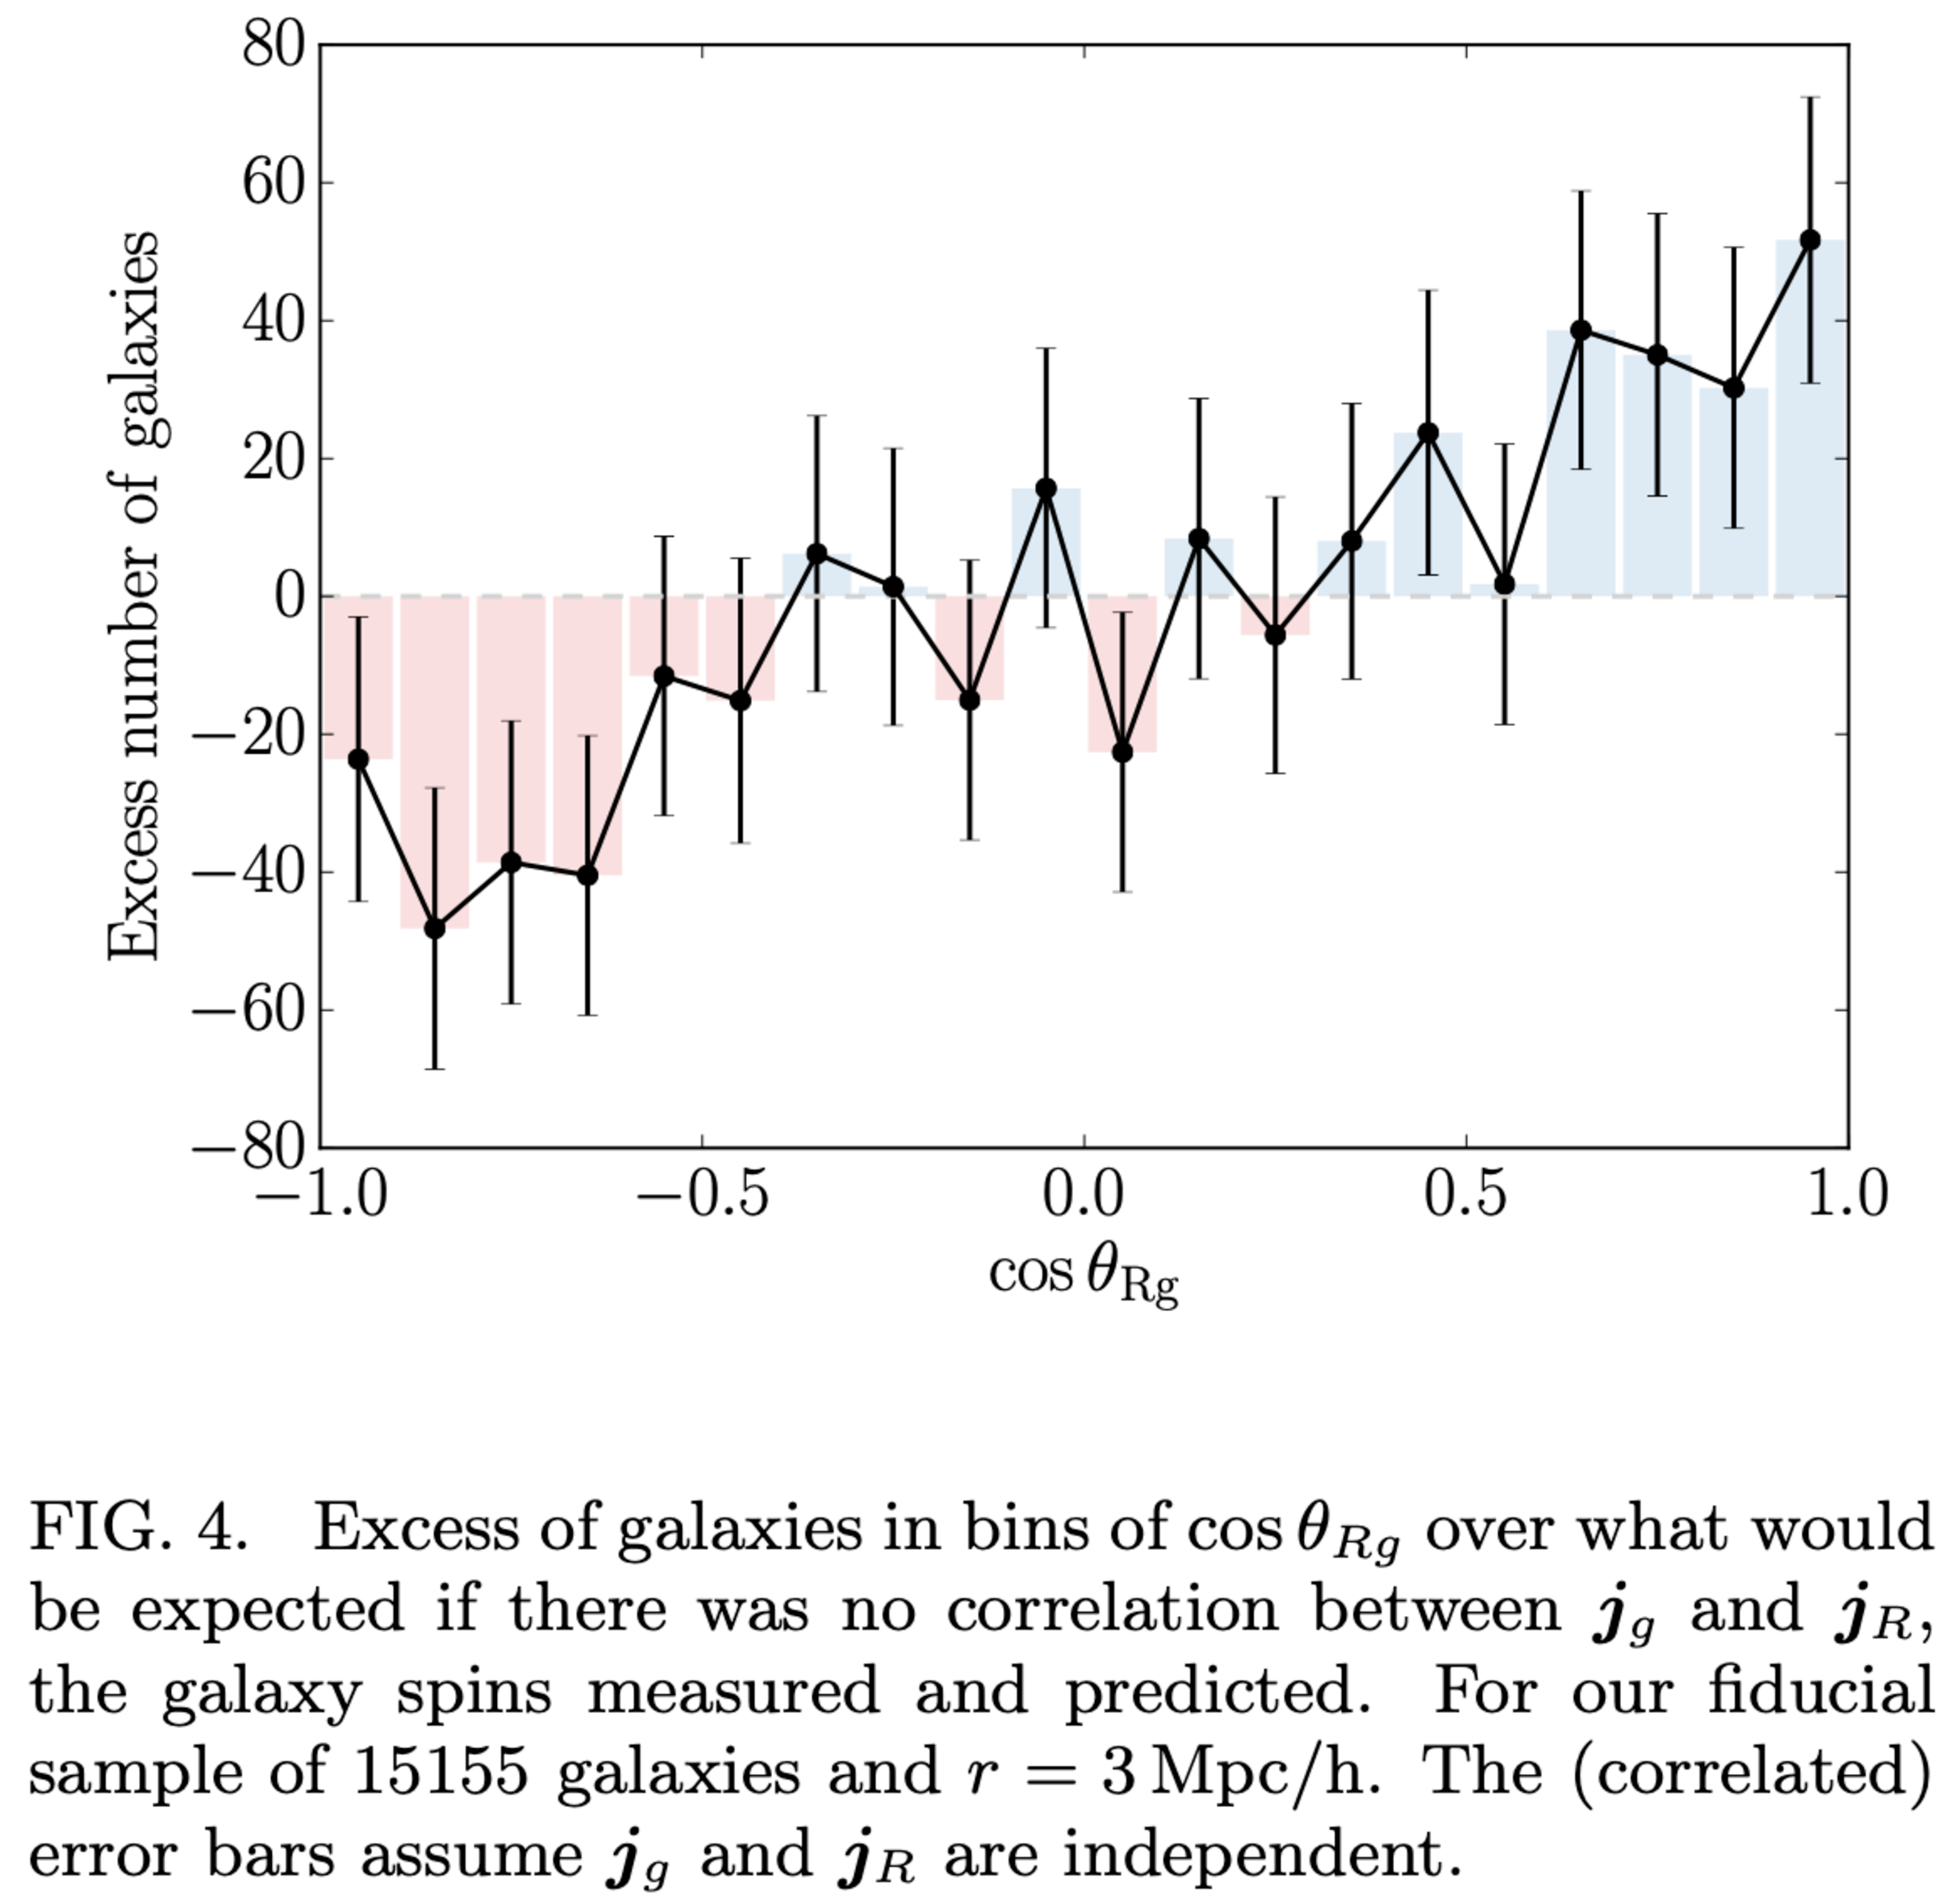
\includegraphics[width=2.9in]{Figures/spincorr.pdf}  
Motloch+ 2021
  }

 
  \frame{
    \frametitle{E-mode Coordinate}
      reduce 3-D Lagrangian map to 1-D potential ({\it max Zeldovich}):
    \begin{eqnarray}      
{\rm potential\ deformation\ \ \ \ \ }  x^i &=& \xi^\mu \delta^i_\mu + \frac{\partial \phi}{\partial
    \xi^\mu}\delta^{i\mu}\nonumber\\
{\rm dreibein\ \ \ \ \ \  } e^i_\mu &\equiv& \partial x^i / \partial \xi ^ \mu \nonumber\\
 {\rm volume\  element\ \ \ \ }\sqrt{g} &\equiv& \mathrm{det}\left| e^i_\mu\right|\nonumber\\
{\rm mass\ coordinate \ \ \ \ \ }    \rho \sqrt{g}&=&\mathrm{Const.}\nonumber\\
    \partial _\mu (\rho \sqrt{g} e^\mu _i \delta^{i\nu}
    \partial_\nu \dot{\phi})&=&\langle\rho\rangle-\rho \sqrt{g}
\label{eqn:dif}
\end{eqnarray}
Solve Monge-Amp\'ere eqn (\ref{eqn:dif}) using multigrid (Pen 1995):
unique bijective mass coordinate.  See also Tully/Peebles, Mohayaee+, Goldberg, Schmidtfull, Wang+, Seljak,
Zaldarriaga, Hada/Eisenstein, Shi/Brikin/Li+, Jasche+, Sarpa+
}

  
 \frame{
    \frametitle{ELUCID projection}
    \begin{itemize}
      \item Motloch, ULP, Yu 2111.12590
    \item $J^\mathrm{IC}_a=  \epsilon_{abc}
\partial_{bk} \phi^r
\partial_{kc} \rho^r$
    \item  $\mathbb{P}^{L/R}_{ab}(\mathbf{k}) = 
  \frac{1}{2}
  \left[
  \(\delta_{ab} - \hat k_a \hat k_b\) 
  \pm    i \epsilon_{abc} \hat k_c \right] $
    \item   $\tilde J^\mathrm{IC}_{L/R,a}(\mathbf{k}) \equiv
  \mathbb{P}^{L/R}_{ab}(\mathbf{k}) 
  \tilde J^\mathrm{IC}_b(\mathbf{k})$
    \item  $\mu_X = \left\langle 
  \frac{\bs{J}^g}{|\bs{J}^g|}
  \cdot
  \frac{\bs{J}^\mathrm{IC}_X}{|\bs{J}^\mathrm{IC}_X|}
  \right\rangle \ \ \ \ \ X \in \{L, R\}$
\item $\mu_- = \mu_L - \mu_R$
     \end{itemize}
  }


  

  
\frame{
%\vspace{-0.5in}
    \frametitle{Conclusions}
    \begin{itemize}
      \item galaxy spins: new probe of initial conditions at $\sim 1$
        Mpc
      \item direction well conserved from the linear initial conditions
      \item measures tidal twist: quadratic dependence on IC
      \item largest information pool for early universe
      \item predictable from observable displacement field using
        non-linear reconstruction
      \item barotropic reconstruction provides inverse Lagrangian map
      \item computationally straightforward, mass coordinate
            similar to Lagrangian
          \item already observable, scalable to much larger surveys, ML
          \item parity odd field, less likely to be contaminated
          \item unique probes of neutrinos, helicities, etc...
     \end{itemize}
  }


  \frame{
    \frametitle{Gas-DM simulations}
    \vspace{-0.1in}
    \center{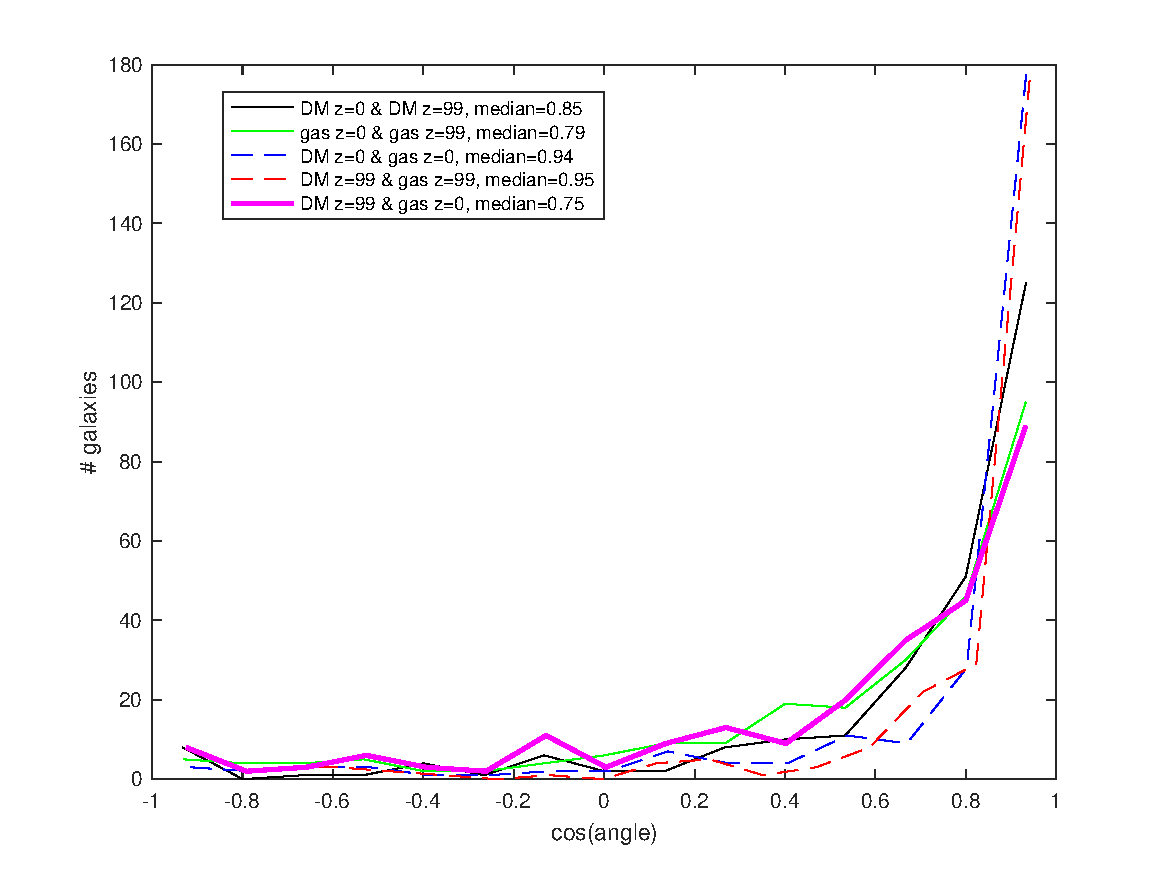
\includegraphics[width=4.01in]{Figures/Illustris_Lagrangian_AM_cosangle_distributions_allgas.pdf}}
    { Shy Genel, Illustris, private communication}
}


\end{document}
